\section{Method}
\label{sec:method}

Let $X=\lbrace x_i\rbrace_{i=1}^{N}$ be the database, $q$ a query, and
$s_i=d(q,x_i)$ a score where smaller is better. Exact flat search computes all
$N$ scores and returns the indices of the $K$ smallest values. Monte-Carlo TopK
keeps the same score matrix but changes the selection step.
Figure~\ref{fig:mc_topk_pipeline} summarizes the data flow.

\begin{figure}[!htbp]
\centering
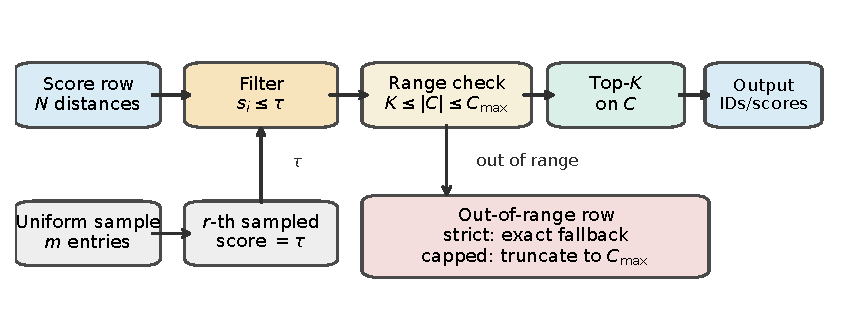
\includegraphics[width=0.88\linewidth]{figures/mc_topk_pipeline.pdf}
\caption{Monte-Carlo TopK is a post-score selector. It samples a threshold,
filters the full score row into a bounded candidate buffer, and runs exact
top-$K$ on the candidates when the count is in range. Out-of-range rows either
fall back to exact selection or use approximate overflow capping.}
\label{fig:mc_topk_pipeline}
\end{figure}

\subsection{Algorithm}

For each query, the algorithm has four stages:

\begin{enumerate}
  \item Select a sample $S \subset \{1,\ldots,N\}$ of size $m$.
  \item Compute or gather sample scores $\{s_i : i \in S\}$ and choose the
        $r$-th smallest sample score as the sampled threshold $\tau$.
  \item Scan the full score row and form the candidate set
        $C=\{i : s_i \leq \tau\}$.
  \item If $K \leq |C| \leq C_{\max}$, where $C_{\max}$ is the candidate buffer
        cap, run exact top-$K$ on $\{s_i : i \in C\}$. If $|C|<K$, fall back to
        exact top-$K$ over all $N$ scores for that row. If $|C|>C_{\max}$,
        either fall back to exact selection or use capped mode, which keeps at
        most $C_{\max}$ candidates and is approximate.
\end{enumerate}

The threshold rank $r$ controls the candidate count. With a uniform sample and
no ties, the threshold quantile is about $r/m$, so the expected candidate count
is about $N r/m$. Useful settings keep this value above $K$ and below the cap.
Larger $r$ reduces underflow risk but keeps more candidates. A larger cap
reduces overflow risk but uses more memory.

Candidate-buffer memory is straightforward. For batch size $Q_{\mathrm{batch}}$,
candidate cap $C_{\max}$, 32-bit scores, and FAISS 64-bit IDs, score/id storage
is about
\[
  Q_{\mathrm{batch}} C_{\max}
  \,(\mathrm{sizeof(float)} + \mathrm{sizeof(idx\_t)})
  \approx 12 Q_{\mathrm{batch}} C_{\max} \text{ bytes}.
\]
For GPU batch size 32, this is about 3.0 MiB at cap 8192, 6.0 MiB at 16384, and
18.3 MiB at 50000, before small counters and output buffers. The cap affects
memory, latency, and accuracy.

For tuning, treat the sampled threshold as a random order statistic. With a
sample of size $m$ drawn without replacement from $N$ unique ranks, the rank
$R_r$ of the $r$-th sample item has
\[
  \mathbb{E}[R_r] = \frac{r(N+1)}{m+1}
  \quad\text{and}\quad
  \mathrm{Var}(R_r) =
  \frac{r(m-r+1)(N+1)(N-m)}{{(m+1)}^2(m+2)}.
\]
The mean alone is insufficient. Underflow means $R_r<K$, or at least $r$ samples landing
among the first $K-1$ population ranks:
\[
  \Pr[c_q<K] =
  \Pr\!\left[\mathrm{Hypergeom}(N,K-1,m) \geq r\right].
\]
Overflow means $R_r>C_{\max}$, or fewer than $r$ samples landing among the
first $C_{\max}$ population ranks:
\[
  \Pr[c_q>C_{\max}] =
  \Pr\!\left[\mathrm{Hypergeom}(N,C_{\max},m) < r\right].
\]

These equations give a starting rule from $N$ and $K$. Choose a candidate
multiplier $\alpha=\mathbb{E}[c]/K$. In exact mode, $\alpha$ should usually be
several times larger than one. For sample size $m$, set
\[
  r \approx \left\lceil \alpha K \frac{m+1}{N+1} \right\rceil
  \approx \left\lceil \alpha K \frac{m}{N} \right\rceil.
\]
If this gives a very small $r$, use a larger $\alpha$ or $m$. For a batch with
$Q$ rows, choose $r$ so that $Q\Pr[c_q<K]\ll 1$. Choose $C_{\max}$ from a high
quantile of $R_r$ under the memory budget, then measure p99 and maximum
candidates in a tuning run. This is a starting range, not a guarantee. Score
ties, finite-precision distances, and query difficulty can change the tails.

The SIFT1M measurements follow this rule. With $N=10^6$, $K=64$, and $m=8192$,
$r=4$ gives about 488 expected candidates and predicts about 18 underflows over
9984 queries. The measured run has 18 fallback rows. Raising $r$ to 8 roughly
doubles the candidates and removes fallbacks. For $K=1024$, the same sample
size needs \texttt{sample\_k=32}. The experiments report underflow, overflow,
and fallback counters with every result.

\subsection{Result Checks}

Let $\gamma_K$ be the $K$-th smallest full-row score. If
$K \leq |C| \leq C_{\max}$, then $\tau \geq \gamma_K$. Exact top-$K$ on $C$
returns the same $K$-th score, $\gamma_K$. If there are no ties at $\gamma_K$,
the returned IDs also match
full-row exact top-$K$. With ties, several ID sets can be valid, so ID overlap
can be below 1.0 even when the score is correct.

Exact mode falls back when fewer than $K$ scores pass, or when more than
$C_{\max}$ scores pass. Results must report underflow, overflow, fallback
count, ID overlap, and the returned $K$-th score. Tie-aware overlap explains
low ID overlap when many vectors share the exact $K$-th score.

Overflow capping is different from threshold filtering. If $|C|>C_{\max}$,
capped mode keeps only $C_{\max}$ candidates and does not fall back. This is
faster, but it can return a worse $K$-th score. It must report overlap against
exact top-$K$.

\subsection{Cost Compared With Exact Selection}

For $Q$ queries, dimension $D$, database size $N$, sample size $m$, output size
$K$, and candidate count $c_q=|C_q|$, full distance computation costs
\[
  T_{\mathrm{dist}} = \Theta(QND).
\]
Exact flat search then runs a full-row selector. A heap-style selector costs
$O(N\log K)$ per query. GPU selectors can be faster, but they still read the
full score row. Let the exact selection cost be
\[
  T_{\mathrm{exact-select}} = \Theta(Q\,S(N,K)),
\]
where $S(N,K)$ is the cost of exact top-$K$ over $N$ scores for a given code
path.

Monte-Carlo TopK adds sampling, one full filter scan, and a smaller candidate
selector:
\[
  T_{\mathrm{MC-select}} =
  \Theta(Q\,S(m,r)) + \Theta(QN) +
  \sum_{q=1}^{Q}\Theta(S(c_q,K)) + T_{\mathrm{fallback}}.
\]
If sample distances are computed separately, the method also pays
$\Theta(QmD)$. If the full score row is already stored, this becomes a gather
over $m$ scores. In flat search, $\Theta(QND)$ remains unchanged:
\[
  T_{\mathrm{MC-flat}} =
  \Theta(QND) + \Theta(QmD) + T_{\mathrm{MC-select}}.
\]

This is not a claim of lower distance cost. A speedup needs
\[
  S(N,K) \gg S(m,r) + N + \mathbb{E}[S(c_q,K)],
\]
with small fallback cost. If distance computation takes most of the time,
end-to-end speedup is limited. With overflow capping, $S(c_q,K)$ is replaced by
$S(\min(c_q,C_{\max}),K)$, but rows with $c_q>C_{\max}$ become approximate.

\subsection{Fallback Avoidance}

Fallbacks are rare but expensive. Underflow means $c_q<K$; overflow means
$c_q>C_{\max}$. The experiments use three safeguards:

\begin{enumerate}
  \item Choose the threshold rank so the expected candidate count is several
        times larger than $K$, not just equal to $K$.
  \item Set the candidate cap using high-percentile candidate counts from a
        tuning run, not only the mean.
  \item Report fallback counts for every speed result, because a few slow
        fallback rows can take most of the total selector time.
\end{enumerate}

Table~\ref{tab:faiss_sift1m} shows the effect. A setting with 18 fallback rows
is slower than exact top-$K$. A safer threshold with zero fallbacks gives nearly
10x selector speedup.
